\section{Differenciālā mērīšanas metode}

Lielākā daļa osciloskopu \cite{tiepie_diffmes} ir viena ieejas puse vienmēr ir savienota ar zemi, bet otra puse ar interesējošo punktu elektriskajā ķēdē.
\begin{figure}[H]
	\centering
    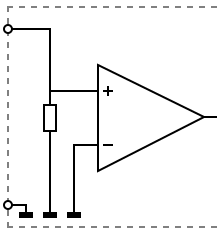
\includegraphics[width=0.5\textwidth]{pictures/osc_1_probe.png}\hspace{1cm}
    \caption{Osciloskopa izvada struktūra}
\end{figure}

Tāpēc spriegums, ko mēra ar osciloskopu, vienmēr tiek mērīts starp konkrēto punktu un zemi. Kad mērāmā ķēde ir savienota ar to pašu references punktu, tad var izveidoties īssavienojums, kas var sabojāt ķēdes daļu un osciloskopu. Lai no tā izvairītos, tiek mērīti vēlamie elektriskie ķēdes posmi ar differenciālo metodi. Šī metode aprēķina sprieguma starpību starp diviem punktiem. Lielākajā daļā osciloskopu to var izdarīt, savienojot vienu no kanāliem ar vienu punktu un otru kanālu ar otru punktu un pēc tam izmantojot osciloskopa matemātisko funkciju Ch1 - Ch2, lai parādītu faktisko sprieguma starpību.
\begin{figure}[H]
	\centering
    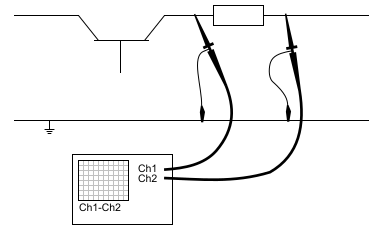
\includegraphics[width=0.5\textwidth]{pictures/osc_2_diff.png}\hspace{1cm}
    \caption{Differenciāla mērīšana izmantojot osciloskopu}
\end{figure}
